%%%%%%%%%%%%%%%%%%%%%%%%%%%%%%%%%%%%%%%%%
% Wenneker Article
% LaTeX Template
% Version 2.0 (28/2/17)
%
% This template was downloaded from:
% http://www.LaTeXTemplates.com
%
% Authors:
% Vel (vel@LaTeXTemplates.com)
% Frits Wenneker
%
% License:
% CC BY-NC-SA 3.0 (http://creativecommons.org/licenses/by-nc-sa/3.0/)
%
%%%%%%%%%%%%%%%%%%%%%%%%%%%%%%%%%%%%%%%%%

%----------------------------------------------------------------------------------------
%	PACKAGES AND OTHER DOCUMENT CONFIGURATIONS
%----------------------------------------------------------------------------------------

\documentclass[10pt, a4paper, twocolumn]{article} % 10pt font size (11 and 12 also possible), A4 paper (letterpaper for US letter) and two column layout (remove for one column)

    %%%%%%%%%%%%%%%%%%%%%%%%%%%%%%%%%%%%%%%%%
% Wenneker Article
% Structure Specification File
% Version 1.0 (28/2/17)
%
% This file originates from:
% http://www.LaTeXTemplates.com
%
% Authors:
% Frits Wenneker
% Vel (vel@LaTeXTemplates.com)
%
% License:
% CC BY-NC-SA 3.0 (http://creativecommons.org/licenses/by-nc-sa/3.0/)
%
%%%%%%%%%%%%%%%%%%%%%%%%%%%%%%%%%%%%%%%%%

%----------------------------------------------------------------------------------------
%	PACKAGES AND OTHER DOCUMENT CONFIGURATIONS
%----------------------------------------------------------------------------------------

\usepackage[english]{babel} % English language hyphenation

\usepackage{microtype} % Better typography

\usepackage{amsmath,amsfonts,amsthm} % Math packages for equations

\usepackage[svgnames]{xcolor} % Enabling colors by their 'svgnames'

\usepackage[hang, small, labelfont=bf, up, textfont=it]{caption} % Custom captions under/above tables and figures

\usepackage{booktabs} % Horizontal rules in tables

\usepackage{lastpage} % Used to determine the number of pages in the document (for "Page X of Total")

\usepackage{graphicx} % Required for adding images

\usepackage{enumitem} % Required for customising lists
\setlist{noitemsep} % Remove spacing between bullet/numbered list elements

\usepackage{sectsty} % Enables custom section titles
\allsectionsfont{\usefont{OT1}{phv}{b}{n}} % Change the font of all section commands (Helvetica)

%----------------------------------------------------------------------------------------
%	MARGINS AND SPACING
%----------------------------------------------------------------------------------------

\usepackage{geometry} % Required for adjusting page dimensions

\geometry{
	top=1cm, % Top margin
	bottom=1.5cm, % Bottom margin
	left=2cm, % Left margin
	right=2cm, % Right margin
	includehead, % Include space for a header
	includefoot, % Include space for a footer
	%showframe, % Uncomment to show how the type block is set on the page
}

\setlength{\columnsep}{7mm} % Column separation width

%----------------------------------------------------------------------------------------
%	FONTS
%----------------------------------------------------------------------------------------

\usepackage[T1]{fontenc} % Output font encoding for international characters
\usepackage[utf8]{inputenc} % Required for inputting international characters

\usepackage{XCharter} % Use the XCharter font

%----------------------------------------------------------------------------------------
%	HEADERS AND FOOTERS
%----------------------------------------------------------------------------------------

\usepackage{fancyhdr} % Needed to define custom headers/footers
\pagestyle{fancy} % Enables the custom headers/footers

\renewcommand{\headrulewidth}{0.0pt} % No header rule
\renewcommand{\footrulewidth}{0.4pt} % Thin footer rule

\renewcommand{\sectionmark}[1]{\markboth{#1}{}} % Removes the section number from the header when \leftmark is used

%\nouppercase\leftmark % Add this to one of the lines below if you want a section title in the header/footer

% Headers
\lhead{} % Left header
\chead{\textit{\thetitle}} % Center header - currently printing the article title
\rhead{} % Right header

% Footers
\lfoot{} % Left footer
\cfoot{} % Center footer
\rfoot{\footnotesize Page \thepage\ of \pageref{LastPage}} % Right footer, "Page 1 of 2"

\fancypagestyle{firstpage}{ % Page style for the first page with the title
	\fancyhf{}
	\renewcommand{\footrulewidth}{0pt} % Suppress footer rule
}

%----------------------------------------------------------------------------------------
%	TITLE SECTION
%----------------------------------------------------------------------------------------

\newcommand{\authorstyle}[1]{{\large\usefont{OT1}{phv}{b}{n}\color{DarkRed}#1}} % Authors style (Helvetica)

\newcommand{\institution}[1]{{\footnotesize\usefont{OT1}{phv}{m}{sl}\color{Black}#1}} % Institutions style (Helvetica)

\usepackage{titling} % Allows custom title configuration

\newcommand{\HorRule}{\color{DarkGoldenrod}\rule{\linewidth}{1pt}} % Defines the gold horizontal rule around the title

\pretitle{
	\vspace{-30pt} % Move the entire title section up
	\HorRule\vspace{10pt} % Horizontal rule before the title
	\fontsize{32}{36}\usefont{OT1}{phv}{b}{n}\selectfont % Helvetica
	\color{DarkRed} % Text colour for the title and author(s)
}

\posttitle{\par\vskip 15pt} % Whitespace under the title

\preauthor{} % Anything that will appear before \author is printed

\postauthor{ % Anything that will appear after \author is printed
	\vspace{10pt} % Space before the rule
	\par\HorRule % Horizontal rule after the title
	\vspace{20pt} % Space after the title section
}

%----------------------------------------------------------------------------------------
%	ABSTRACT
%----------------------------------------------------------------------------------------

\usepackage{lettrine} % Package to accentuate the first letter of the text (lettrine)
\usepackage{fix-cm}	% Fixes the height of the lettrine

\newcommand{\initial}[1]{ % Defines the command and style for the lettrine
	\lettrine[lines=3,findent=4pt,nindent=0pt]{% Lettrine takes up 3 lines, the text to the right of it is indented 4pt and further indenting of lines 2+ is stopped
		\color{DarkGoldenrod}% Lettrine colour
		{#1}% The letter
	}{}%
}

\usepackage{xstring} % Required for string manipulation

\newcommand{\lettrineabstract}[1]{
	\StrLeft{#1}{1}[\firstletter] % Capture the first letter of the abstract for the lettrine
	\initial{\firstletter}\textbf{\StrGobbleLeft{#1}{1}} % Print the abstract with the first letter as a lettrine and the rest in bold
}

%----------------------------------------------------------------------------------------
%	BIBLIOGRAPHY
%----------------------------------------------------------------------------------------

\usepackage[backend=bibtex,style=authoryear,natbib=true]{biblatex} % Use the bibtex backend with the authoryear citation style (which resembles APA)

\addbibresource{example.bib} % The filename of the bibliography

\usepackage[autostyle=true]{csquotes} % Required to generate language-dependent quotes in the bibliography


%----------------------------------------------------------------------------------------
%	Listing
%----------------------------------------------------------------------------------------

\usepackage{listings}
\lstset{ 
    basicstyle=\color[RGB]{169,183,198}\small,
	commentstyle=\color[RGB]{96,139,78},
    stringstyle=\rmfamily\slshape\color[RGB]{96,139,78},	
    keywordstyle=\color[RGB]{190,120,50}\bfseries,
    breaklines=true,
    %行号
    numbers=left,
    rulesepcolor=\color{red!20!green!20!blue!20},
    escapeinside=``,
    xleftmargin=2em,xrightmargin=2em, aboveskip=1em,
    %背景框
    framexleftmargin=1.5mm,
    frame=shadowbox,
    %背景色
    backgroundcolor=\color[RGB]{43,43,43},
    %样式
    % keywordstyle=\color{blue}\bfseries,
    identifierstyle=\color[RGB]{255,198,109},
    numberstyle=\color[RGB]{0,192,192},
    % commentstyle=\it\color[RGB]{96,96,96},
    %显示空格
    showstringspaces=false
} % Specifies the document structure and loads requires packages
    
    %----------------------------------------------------------------------------------------
    %	ARTICLE INFORMATION
    %----------------------------------------------------------------------------------------
    
    \title{Lab report for CA Lab2} % The article title
    
    \author{
        \authorstyle{Xiangzhe Xu} % Authors
        \newline\newline % Space before institutions
        \institution{Nanjing University}\\ % Institution 1
    }
    
    % Example of a one line author/institution relationship
    %\author{\newauthor{John Marston} \newinstitution{Universidad Nacional Autónoma de México, Mexico City, Mexico}}
    
    \date{\today} % Add a date here if you would like one to appear underneath the title block, use \today for the current date, leave empty for no date
    
    %----------------------------------------------------------------------------------------
    
    \begin{document}
    
    \maketitle % Print the title
    
    \thispagestyle{firstpage} % Apply the page style for the first page (no headers and footers)
    
    %----------------------------------------------------------------------------------------
    %	ABSTRACT
    %----------------------------------------------------------------------------------------
    
    \lettrineabstract{This
        is the report of the CA Lab2.
        In this lab, students are required to analyze the performance of "cmove" instruction
        under different branch patterns and branch predictors. 
    }
    
    %----------------------------------------------------------------------------------------
    %	ARTICLE CONTENTS
    %----------------------------------------------------------------------------------------
    
    \section{CMOV}
    %----------------------------------------------------------------------------------------
    \subsection{Brief introduction}
    The CMOVcc instructions check the state of one or more of the status flags in the EFLAGS 
    egister (CF, OF, PF, SF, and ZF) and perform a move operation if the flags are 
    in a specified state (or condition). A condition code (cc) is associated with each 
    instruction to indicate the condition being tested for. 
    If the condition is not satisfied, a move is not performed and execution continues 
    with the instruction following the CMOVcc instruction.
    \
    The CMOVcc instructions were introduced in P6 family processors; however,
     these instructions may not be supported by all IA-32 processors.
    \footnote{Intel® 64 and IA-32 Architectures Software Developer’s Manual}

    %----------------------------------------------------------------------------------------
    \subsection{Performance on modern processors}
    \begin{figure}[!h]
        \centerline{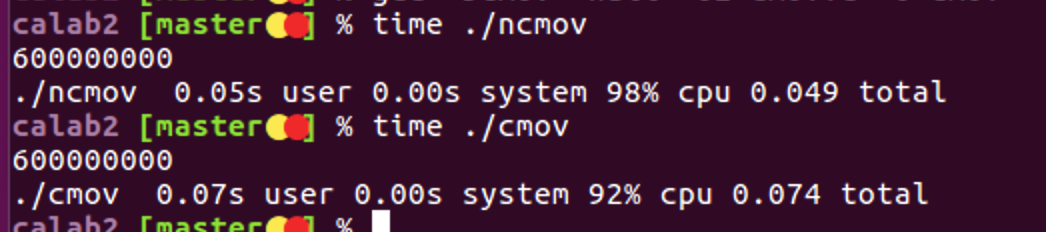
\includegraphics[width=0.5\textwidth]{pics/cmov-branch.png}}
    \end{figure}
    As is shown in the figure, there is hardly any difference between the cmove version and the
    ncmov version, although I have changed the loop times to 10,000,000. It's reasonable to say that
    the cmove instruction would not affect the performance of programs running on a modern processor.
    %----------------------------------------------------------------------------------------
    \section{Preparation}
    %----------------------------------------------------------------------------------------
    \subsection{Patch file}
    The patch file (also called a patch for short) is a text file that consists of 
    a list of differences and is produced by running the related \textbf{\texttt{diff}} program with the 
    original and updated file as arguments. Updating files with patch is often referred to
     as applying the patch or simply patching the files.
    %----------------------------------------------------------------------------------------
    \subsection{Source code analysis}
    \begin{lstlisting}[language=C]
#define choose(i, a, b) ({	\
unsigned long result;	\
asm("testl %1,%2 ; cmovne %3,%0" \
    :"=r" (result)	\
    :"i" (BIT),	\
        "g" (i),	\
        "rm" (a),	\
        "0" (b));	\
result; })
    \end{lstlisting}
    This is the CMOV version macro in cmov.c, which means that result is the output of this 
    assemble sentence and is readonly. Also, the variable i should be placed in a general register and 
    variable a should be placed in either memory or register. Finally, the variable b is the same with 
    the 0th variable. 
    \begin{lstlisting}[language=C]
#define choose(i, a, b) ({		\
unsigned long result;		\
asm("testl %1,%2 ; je 1f ; mov %3,%0\n1:"	\
:"=r" (result)		\
:"i" (BIT),		\
    "g" (i),		\
    "g" (a),		\
    "0" (b));		\
result; })

#endif
        
    \end{lstlisting}
    The not-cmov version is similar with the above one. 
    %----------------------------------------------------------------------------------------
    \section{WorkFlow}
    %----------------------------------------------------------------------------------------
    \subsection{Bash script}
    \begin{lstlisting}[language=C]
CONFIG="--cmd=lab2/cmov1 --cpu-type=DerivO3CPU --caches --l2cache --bpred=LocalBP"

build/X86/gem5.opt configs/example/se.py ${CONFIG}

FILE_NAME=local_1_cmov


mkdir lab2/ret/${FILE_NAME}

echo ${CONFIG} > config.txt

cp m5out/stats.txt lab2/ret/${FILE_NAME}/stats.txt
        
    \end{lstlisting}
    This is a part of my bash script to generate the result.
    %----------------------------------------------------------------------------------------
    \subsection{Numbers}
    In this lab, I choose to use Numbers as my data processor for there's merely a dozen of result-sets.
    Writing a python script for them is time-consuming. Nevertheless, I use matplotlib to draw the diagrams.
    %----------------------------------------------------------------------------------------
    \section{Result}
    \subsection{Time}
    \subsubsection{Facts}
    
    In terms of running time, the branch version with local predictor consume 
    the longest time. The performance of cmov is significantly higher than
    that of the branch one.
    In contrast, the branch version with tournament predictor even run faster
    than the cmov one.
    It's also interesting to find that the local-branch version is more sensitive
    to BITs than the other version.
    \begin{figure}[!h]
        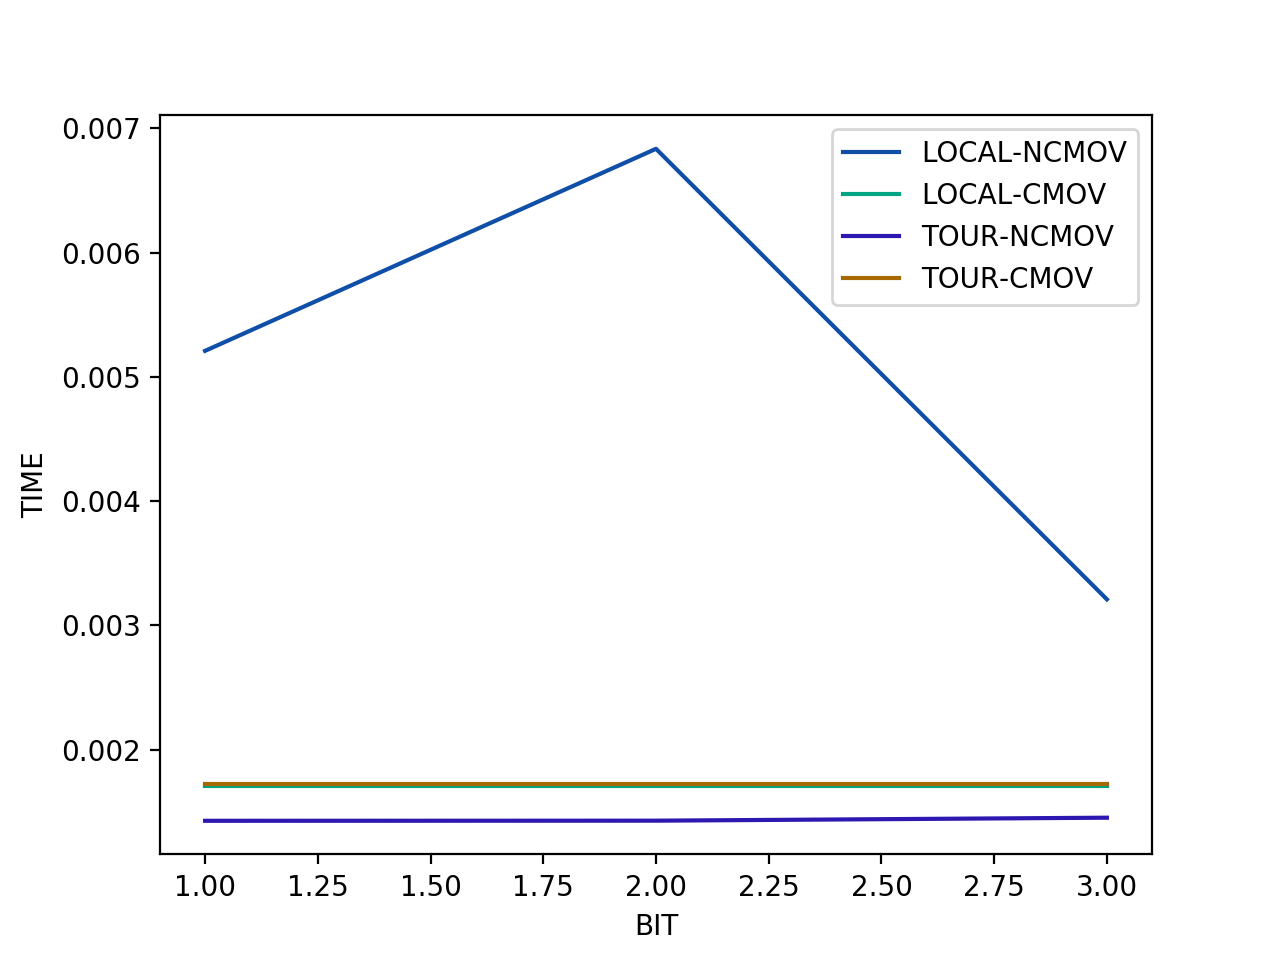
\includegraphics[width=0.5\textwidth]{pics/bit-time.png}
    \end{figure}
    \subsubsection{Analysis}

    
    %------------------------------------------------
    
        
    
    %------------------------------------------------
    
    
    \end{document}
    